\begin{frame}
    \frametitle{Restbudget}    
	\begin{figure}
		\centering
		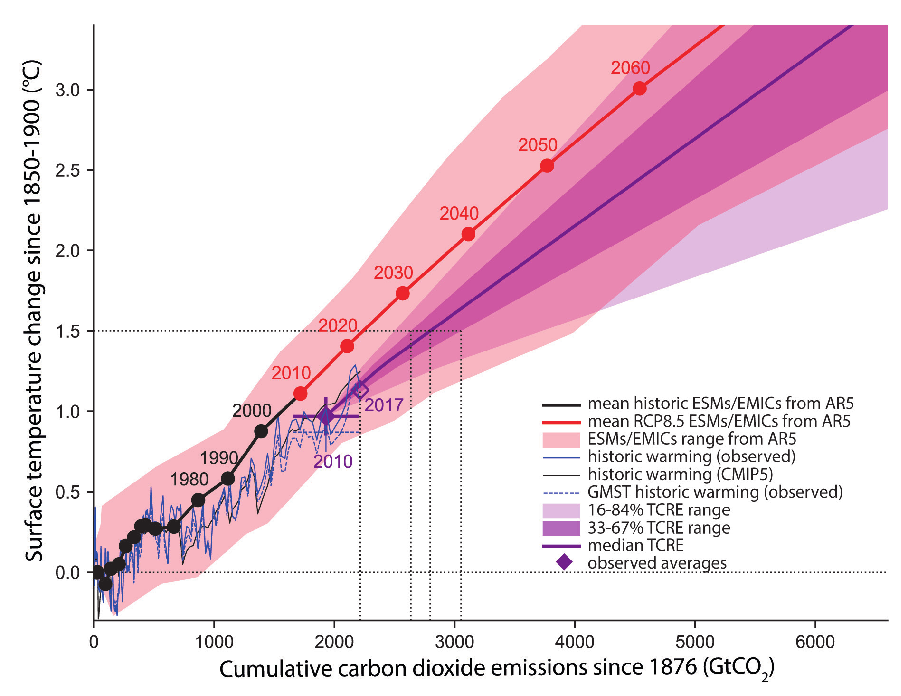
\includegraphics[height=.6\textheight]{bilder/cumulative_co2.pdf}
		\caption{Globale Oberflächentemperatur gegen kumulative CO$_2$-Emissionen.}
    \end{figure}
    
    \begin{itemize}
        \item Menge verbleibender Emissionen zur Begrenzung der Temperaturerhöhung
        \item Auf Basis von RCP8.5 Szenario des IPCC (business-as-usual)
        \item Auf Basis von Szenarien, die die globale Erderwärmung bis 2100 auf 1,5°C erreichen
    \end{itemize}
\end{frame}

\begin{frame}
	\frametitle{CO$_2$ Restbudget für Erwärmung um 1,5°C}
    \begin{itemize}
        \item Emission von maximal 420 GtCO$_2$ zur Einhaltung mit 66\%iger Warscheinlichkeit
        \item Emission von maximal 580 GtCO$_2$ zur Einhaltung mit 50\%iger Warscheinlichkeit
        \item Reduktion um 100 GtCO$_2$ bei Berücksichtigung von Erdsystem-Rückkopplungen wie Auftauen von Permafrostböden
        \item Globale Emissionen in 2019 49 GtCO$_2$eq % https://edgar.jrc.ec.europa.eu/overview.php?v=booklet2019
        \item Bei gleichgbleibender Rate sind die Restbudgets in 8,5 bzw. 11,8 Jahren aufgebraucht
    \end{itemize}

	\note{
		\begin{itemize}
			\item Restbudgets einerseits aus Erwärmung im Vergleich zu 1861-1880 auf Basis des RCP8.5 Szenarios
            \item Andererseits \"from a set of available pathways that were assessed to have a >50\% probability to exceed 1.5°C by mid-century, and return to 1.5°C or below in 2100 with greater than 66\% probability\"
            \item Weitere Studien, die teilweise nur CO$_2$ berücksichtigen
            \item Seit dem AR5 Report 2014 viele weitere Veröffentlichungen, die berücksichtigt werden
            \item Viele Unsicherheiten auf die berechneten Restbudgets wie Unterschiede in Szenarien zur Entwicklung von nicht-CO$_2$ Emissionen oder die Unsicherheit auf die historische Temperatur von 1850-1900
		\end{itemize}
	}
\end{frame}

\begin{frame}
    \frametitle{CO$_2$-Emissionen Deutschlands}
	\begin{figure}
		\centering
		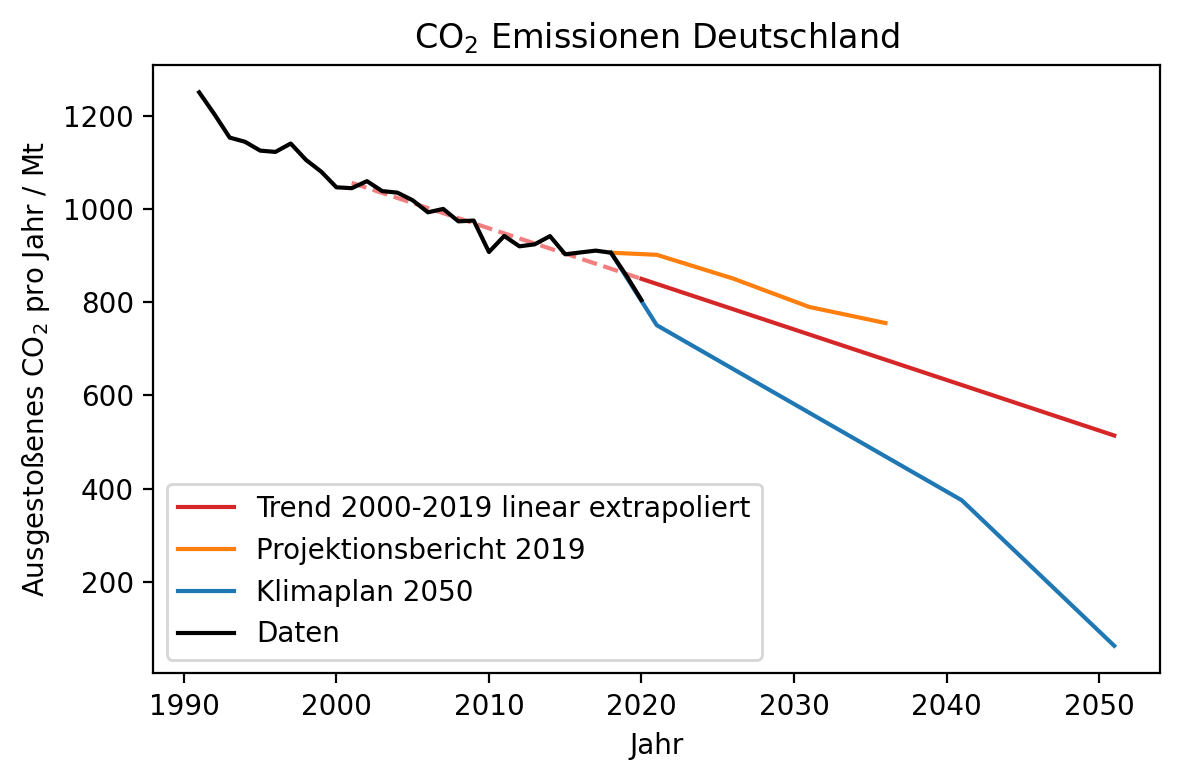
\includegraphics[height=.55\textheight]{bilder/co2-emissions-de.png}
		\caption{CO$_2$-Emissionen.}
    \end{figure}
    \begin{itemize}
        \item Bei Fortsetzung des linearen Trends würde das Ziel "0-Emissionen" erst in ca. 80 Jahren erreicht.
        \item Der Projektionsbericht der Bundesregierung 2019 zeigt, dass die deutschen Anstrengungen zum Klimaschutz nicht zielführend sind.
        \item Klimaplan 2050 auf Basis des Pariser Abkommens zeigt einen ambitionierten Weg, aber es ist unklar, wie dieser gegangen werden soll.
    \end{itemize}
\end{frame}

\begin{frame}
    \frametitle{Wie viele Emissionen stehen Deutschland noch zu?}
	\begin{figure}
		\centering
		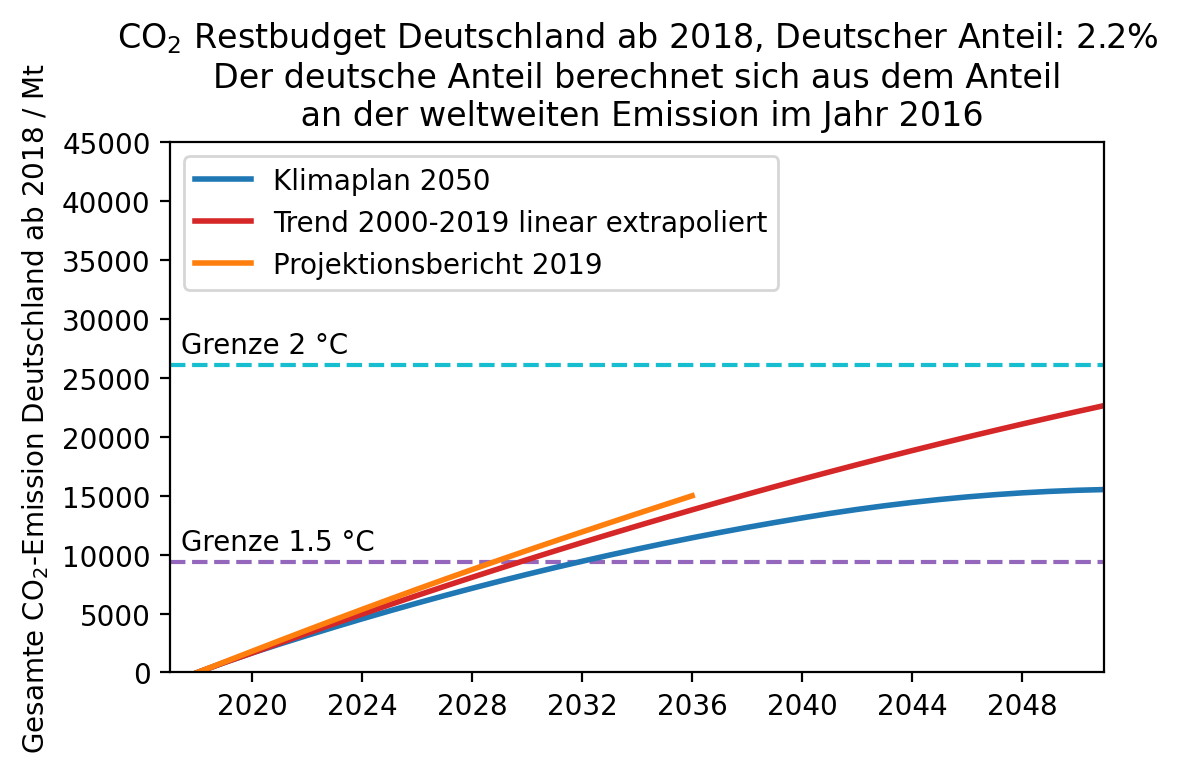
\includegraphics[height=.6\textheight]{bilder/restbudget_de_new.png}
		\caption{Globale Oberflächentemperatur gegen kumulative CO$_2$-Emissionen.}
    \end{figure}
    \begin{itemize}
        \item Die Bundesregierung geht davon aus, dass Deutschland aus den globalen CO2-Budgets, die vom IPCC errechnet wurden ca. 2.2\% zustehen.
        \item Danach darf Deutschland pro Kopf doppelt so viel CO2 ausstoßen, wie der durchschnittliche CO2-Ausstoß pro Person auf der Welt ist.
    \end{itemize}
    
\end{frame}
